\chapter{Analisi delle performance}
In questo capitolo si analizza il comportamento del sistema sotto diverse configurazioni.\\

Per ottenere un'analisi del sistema maggiormente affidabile � stata tolta la parte di visualizzazione grafica, poich� andrebbe ad alterare i risultati in quanto richiede un tempo maggiore per poter essere creata e modificata.

\section{Classe Config}
Per settare le varie configurazioni del sistema il programma presenta una classe nella quale sono presenti tutte le costanti per modificarne il funzionamento.
Tra cui il numero di particelle, il numero di step, il numero di thread e altre costanti.
In particolare settando ``ALL\_PARTICLES\_EQUALS'' a true si assegna a tutte le particella un'alfa e una massa costanti che altrimenti sarebbero generati casualmente per ogni particella.
\section{SpeedUp}

\index{Titolo per indice della sezione}
Il sistema � stato testato con due configurazioni differenti: nel primo caso utilizzando 1000 particelle, ovvero sottoponendo il sistema ad un carico computazionale oneroso.
Nella seconda configurazione si utilizzano 100 particelle, di conseguenza un carico computazionale notevolmente inferiore.\\
In entrambi i casi il sistema � stato eseguito cambiando il numero di step e per ciascuno anche il numero di thread.
\newpage
\subsection{Configurazione con 1000 particelle}
\begin{figure}[!h]
    {\begin{center}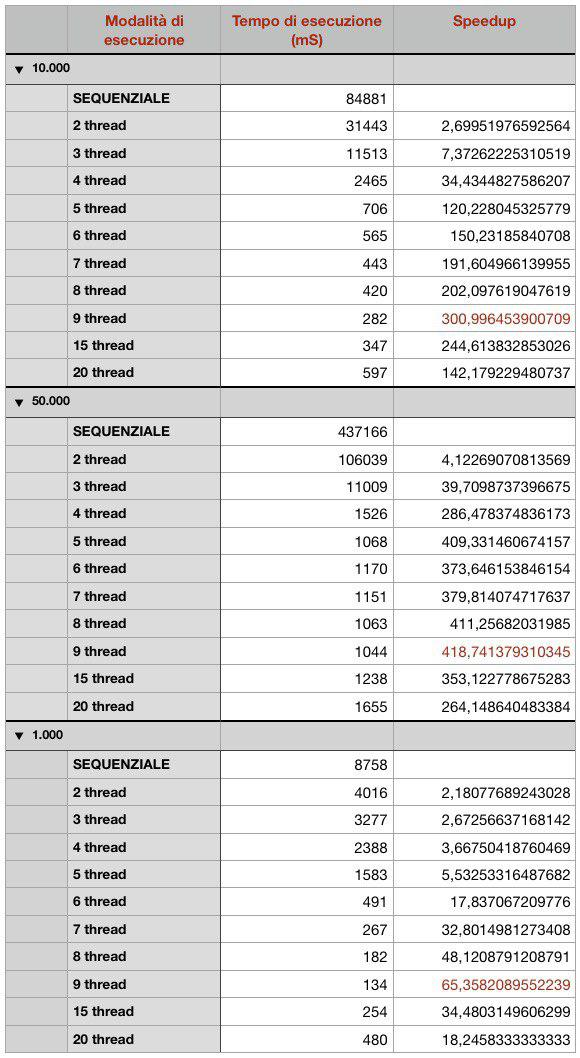
\includegraphics[width=8cm]{FIGURE/tab1.jpg}\end{center}}
\caption{Configurazione con 1000 particelle \label{tab1}}
\end{figure}
Come si evince dalla tabella \ref{tab1} il valore dello speed up continua a crescere aumentando il numero di thread in esecuzione, fino ad un massimo di thread pari al numero di processori della macchina pi� uno (nel nostro caso equivale a 9 threads).
\newpage
\subsection{Configurazione con 100 particelle}
\begin{figure}[!h]
    {\begin{center}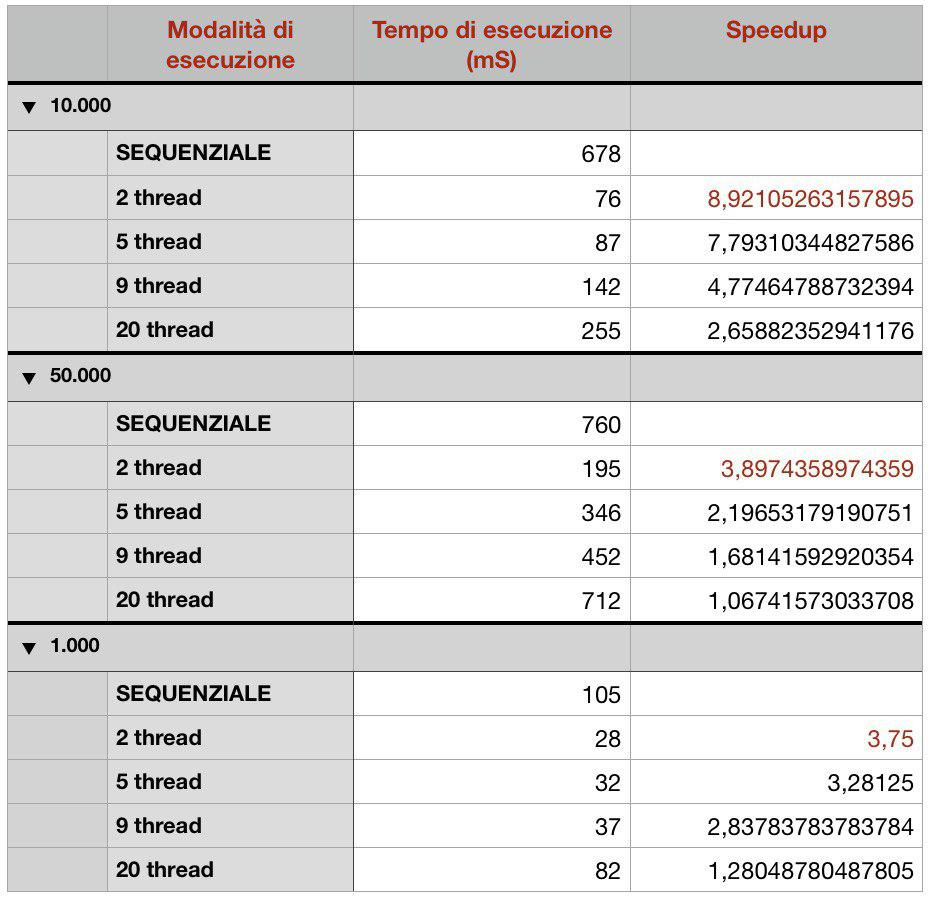
\includegraphics[width=12cm]{FIGURE/tab2.jpg}\end{center}}
\caption{Configurazione con 100 particelle \label{tab2}}
\end{figure}
In questo secondo caso la tabella \ref{tab2} mostra che lo speed up migliore � ottenuto con un numero inferiore di threads rispetto al caso precedente, poich�, probabilmente, il cambio di contesto dovuto all'esecuzione dei diversi threads causa un costo pi� elevato rispetto ad un esecuzione che comporta una maggiore sequenzializzazione.